\section{\textbf{Results}}

This study employed a quantitative within-subjects design examining three primary dependent variables: effectiveness ratings (participants' evaluations of assistance conditions on five-point Likert scales), revision frequency (number of iterative prompt modifications), and time on task (task completion duration). The analytical approach prioritized non-parametric methods due to violations of normality assumptions, employing the Friedman test for omnibus comparisons, Wilcoxon signed-rank tests with Bonferroni correction for pairwise analyses, and Spearman's rank correlation for associational patterns. Results indicated significant departures from normality across all conditions ($p < 0.001$ for all four conditions), violating parametric test assumptions. Supplementary D'Agostino-Pearson and Jarque-Bera tests corroborated these findings, though the control condition showed mixed outcomes across different normality metrics.

\subsection{\textbf{Preliminary Analysis}}

\subsubsection{Normality Assessment:}

Prior to selecting appropriate statistical tests, distributional assumptions were evaluated using multiple convergent methods. The Shapiro-Wilk test, recognized for its superior statistical power in detecting deviations from normality compared to alternatives such as Kolmogorov-Smirnov, was applied to effectiveness scores across all four assistance conditions with 99 observations each (33 participants × 3 tasks).

\begin{figure}[h]
\centering
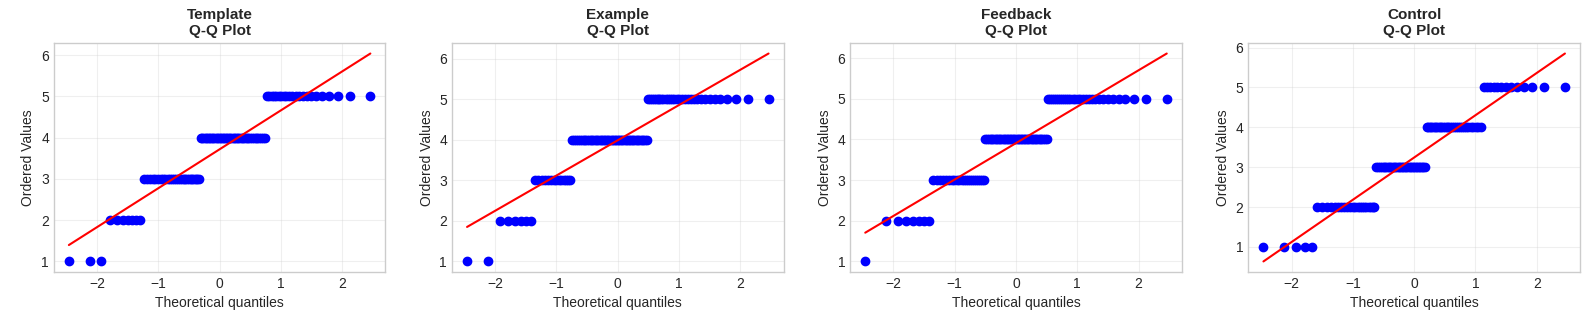
\includegraphics[width=0.9\textwidth]{figures/01.png}
\caption{Q-Q Plots of Effectiveness Scores Across Assistance Conditions}
\label{fig:qq_plots}
\end{figure}

Visual diagnostics reinforced the statistical findings. Q-Q (Quantile–Quantile) plots \autoref{fig:qq_plots} revealed systematic deviations from the reference line across all conditions, with notable clustering around middle ranges and departures at distributional extremes.  

\begin{figure}[h]
\centering
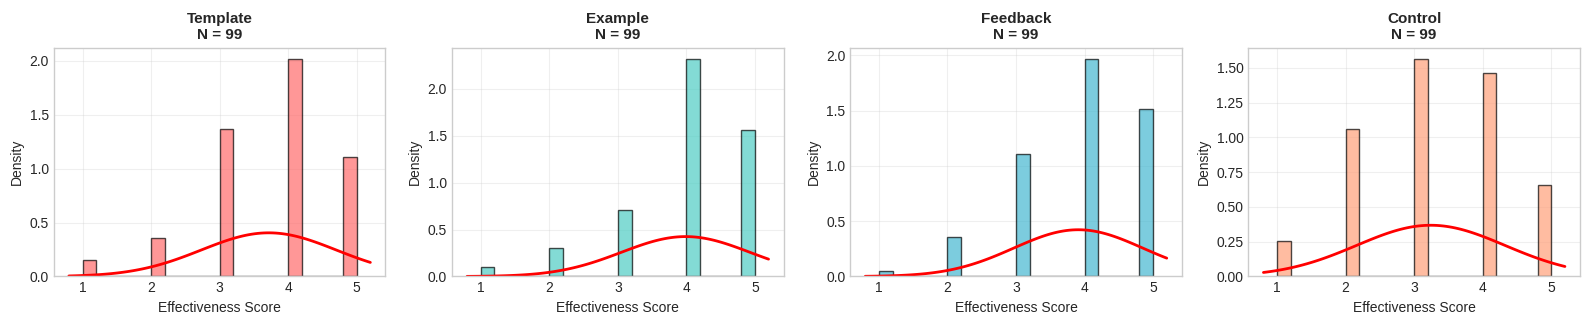
\includegraphics[width=0.9\textwidth]{figures/02.png}
\caption{Histograms of Effectiveness Scores Across Assistance Conditions}
\label{fig:histograms}
\end{figure}

Histograms with overlaid normal density curves \autoref{fig:histograms} demonstrated substantial divergence from theoretical normal distributions, exhibiting pronounced skewness and concentration at specific scale values. Example-based and feedback-based conditions showed heavy clustering at upper scores (4 and 5), while the control-based displayed greater dispersion around lower central values.

\begin{figure}[h]
\centering
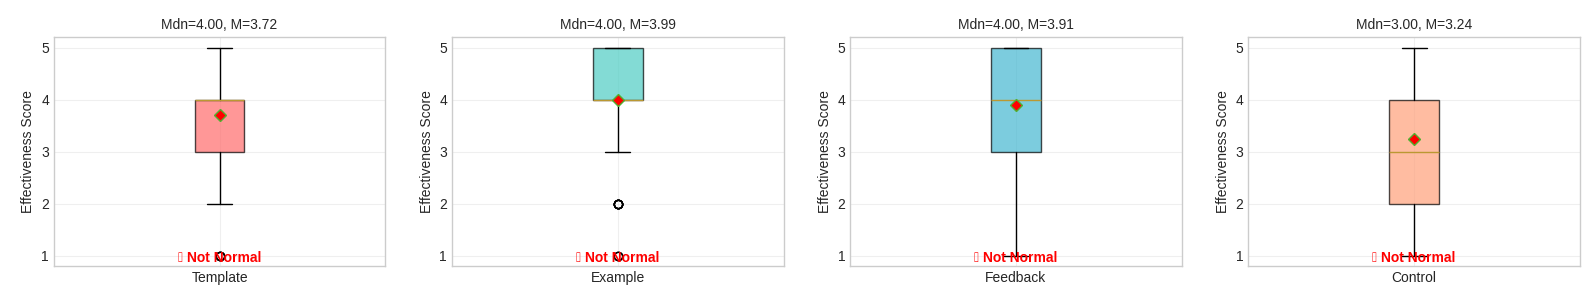
\includegraphics[width=0.9\textwidth]{figures/03.png}
\caption{Boxplots of Effectiveness Scores Across Assistance Conditions}
\label{fig:boxplots}
\end{figure}

Boxplots \autoref{fig:boxplots} further confirmed non-normality through irregular distributional shapes and outlier patterns inconsistent with Gaussian distributions. These convergent findings necessitated the adoption of non-parametric statistical approaches for all subsequent analyses, ensuring robust inference despite distributional violations.

\subsubsection{Descriptive Statistics:}

Central tendency and variability measures were calculated using medians and interquartile ranges (IQRs), preferred for ordinal Likert-scale data over means and standard deviations. \autoref{tab:descriptive_stats} presents comprehensive descriptive statistics for effectiveness ratings across all assistance conditions.

\begin{table}[h]
\centering
\begin{tabular}{lccccccc}
\hline
\textbf{Strategy} & \textbf{Median} & \textbf{Mean} & \textbf{SD} & \textbf{IQR} & \textbf{Min} & \textbf{Max} \\
\hline
Template & 3.67 & 3.72 & 0.78 & [3.33, 4.33] & 2.00 & 5.00 \\
Example & 4.00 & 3.99 & 0.74 & [3.67, 4.33] & 2.00 & 5.00 \\
Feedback & 4.00 & 3.91 & 0.64 & [3.67, 4.33] & 3.00 & 5.00 \\
Control & 3.33 & 3.24 & 0.72 & [3.00, 3.67] & 1.00 & 5.00 \\
\hline
\end{tabular}
\caption{Descriptive Statistics for Effectiveness Ratings by Assistance Condition}
\label{tab:descriptive_stats}
\end{table}

Example-based and feedback-based conditions achieved identical median effectiveness ratings (4.00), with narrow IQRs indicating consistent positive evaluations across participants. Both conditions demonstrated relatively low standard deviations (0.74 and 0.64, respectively), suggesting greater consensus regarding their utility.

Template-based assistance produced moderate effectiveness ratings (median = 3.67, M = 3.72), with a slightly wider distributional spread (IQR = [3.33, 4.33], SD = 0.78) compared to example-based and feedback-based assistance, indicating more variable participant responses.

The control condition yielded the lowest effectiveness evaluations (median = 3.33, M = 3.24), with the widest range (min = 1.00, max = 5.00) but moderate standard deviation (0.72), reflecting substantial between-participant variation in unassisted performance.

\subsection{\textbf{Primary Analysis}}

\subsubsection{Non-Parametric Analysis using the Friedman Test:}

The Friedman test is a non-parametric alternative to repeated measures ANOVA, designed to detect differences across multiple related groups when the assumption of normality is violated, as was the case in our study. It ranks the scores of each subject across conditions and evaluates whether these ranks differ systematically between groups. This repeated measures operates by ranking participant scores within conditions and tests whether rank distributions differ systematically across groups.

\begin{figure}[h]
\centering
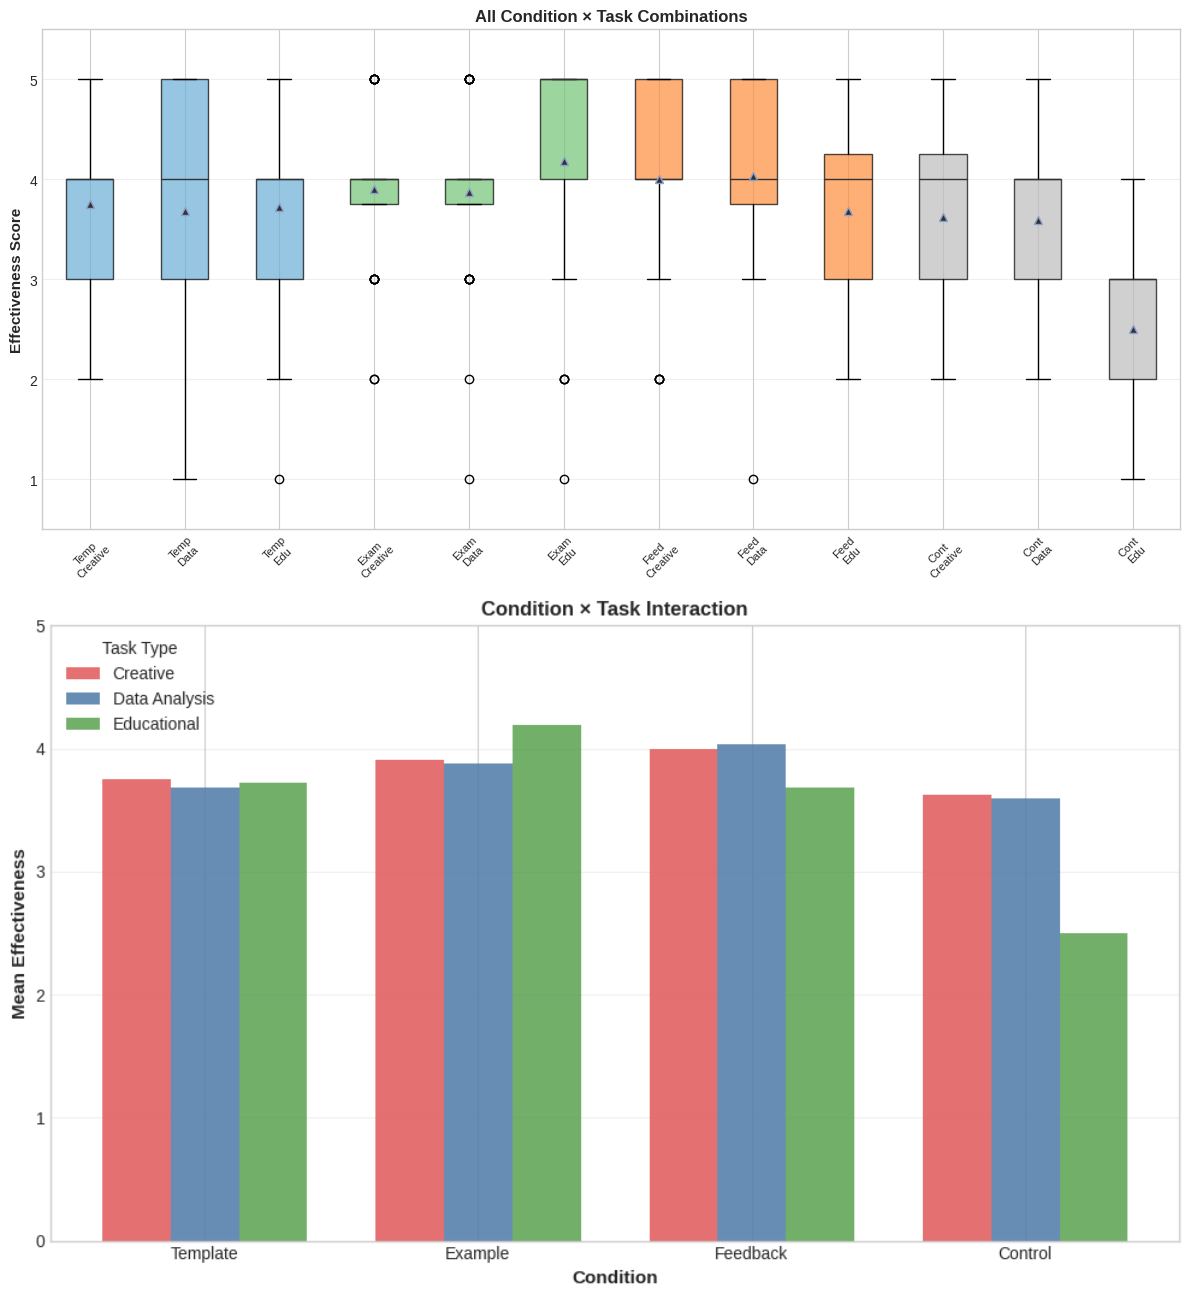
\includegraphics[width=0.6\textwidth]{figures/04.jpg}
\caption{Effectiveness of Assistance Conditions Across Task Domains: Boxplots and Bar Charts (Friedman Test Results)}
\label{fig:effectiveness_domains}
\end{figure}

\autoref{fig:effectiveness_domains} presents the effectiveness results across all condition × task combinations. The boxplots (top panel) illustrate the distribution of scores, while the bar chart (bottom panel) highlights condition × task interactions. Clear differences emerged between assistance conditions. Example-based and feedback-based support consistently produced higher median effectiveness scores, with concentrated ratings at the upper end of the scale, whereas template support yielded moderate improvements and control showed the lowest ratings with greater variability and several outliers. These differences confirm the Friedman test finding that assistance conditions significantly influenced perceived effectiveness.

Breaking the results down by task domain, example-based assistance was most effective in data analysis, where participants rated it highest for guiding them to structure prompts that extracted patterns and insights. Feedback-based assistance was most effective in educational tasks, reflecting its value in iteratively refining explanations for clarity and learner appropriateness. In creative writing, both example-based and feedback-based assistance outperformed template-based and control-based, though the differences were less pronounced compared to the other domains. Template-based support provided steady but modest benefits across all domains, helping participants cover essential details but not reaching the higher effectiveness levels of example-based or feedback-based assistance. By contrast, the control condition consistently underperformed, with the lowest ratings across all three domains, particularly in educational tasks where participants struggled most without guidance.

\subsubsection{Post-hoc Pairwise Comparisons:}

The Wilcoxon signed-rank test is a non-parametric post-hoc procedure that is widely applied after a Friedman test indicates significant differences across multiple conditions \cite{Benavoli2016Should} \cite{Xiang2022Large}. It evaluates whether the distribution of paired differences between two conditions is symmetric around zero by ranking the absolute differences, assigning signs, and testing whether the sum of signed ranks deviates significantly from what would be expected under the null hypothesis of no median difference.

\begin{figure}[h]
\centering
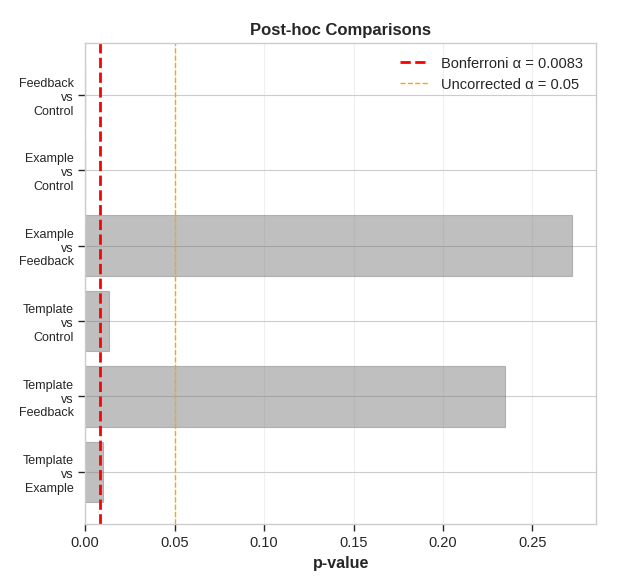
\includegraphics[width=0.7\textwidth]{figures/05.png}
\caption{Post-hoc Wilcoxon signed-rank Comparisons Across Assistance Conditions}
\label{fig:posthoc_wilcoxon}
\end{figure}

Following the significant Friedman test result, pairwise comparisons were conducted using the Wilcoxon signed-rank test, with the Bonferroni correction ($\alpha = 0.0083$) applied to adjust for multiple comparisons by dividing the overall significance level by the number of pairwise tests. The results, shown in \autoref{fig:posthoc_wilcoxon}, revealed that Template vs. Control and Feedback vs. Control both yielded highly significant differences ($p < 0.0083$), indicating that structured support in these conditions substantially improved effectiveness compared to no support. Example-based vs. control-based also showed a significant improvement, further confirming that unassisted prompting was consistently less effective. In contrast, Template vs. Example and Feedback vs. Example did not reach statistical significance, suggesting that although both Example and Feedback performed strongly, their difference was not large enough to be considered statistically reliable. Moreover, Example vs. Feedback produced the largest $p$-value ($> 0.25$), demonstrating clear similarity between these two conditions in terms of user-rated effectiveness. Overall, the post-hoc analysis reinforces the descriptive findings: example-based and feedback-based conditions substantially outperformed control and template-based, but did not differ significantly from each other, highlighting their comparable strength as structured assistance methods.

\subsubsection{Effect Size:}

Effect size measures provide an estimate of the magnitude of differences between conditions, complementing significance testing by indicating the practical importance of results \cite{in2024alternatives}. For Friedman tests, the recommended effect size is Kendall's W, which is calculated as:

\begin{equation}
W = \frac{\chi^2_{F}}{n (k-1)}
\end{equation}

where $\chi^2_{F}$ is the Friedman statistic, $n$ is the number of participants, and $k$ is the number of conditions. Kendall's W ranges from 0 (no agreement) to 1 (perfect agreement), with thresholds of 0.1, 0.3, and 0.5 typically interpreted as small, moderate, and large effects, respectively. In this study, Kendall's $W = 0.332$, indicating a moderate overall effect of the assistance strategy on effectiveness ratings. Reporting Kendall's W alongside significance testing provides interpretable evidence of practical significance \cite{in2024alternatives,tomczak2022need}.

\begin{figure}[h]
\centering
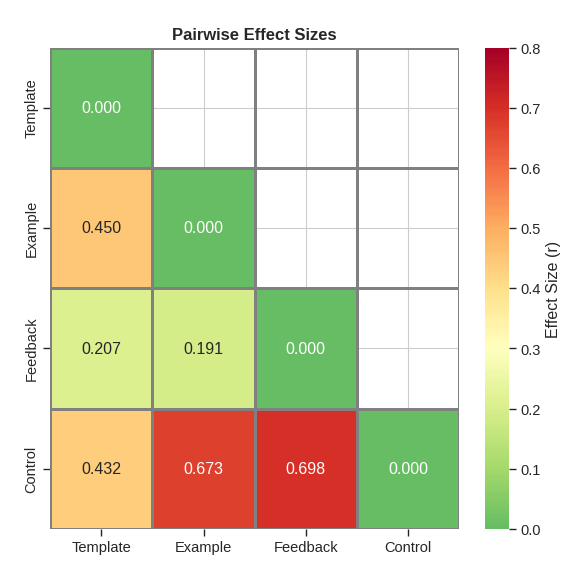
\includegraphics[width=0.6\textwidth]{figures/06.png}
\caption{Pairwise Effect Sizes (Wilcoxon signed-rank r) Across Assistance Conditions}
\label{fig:pairwise_effect_sizes}
\end{figure}

To complement this omnibus effect, pairwise effect sizes were also calculated for the Wilcoxon signed-rank comparisons using the correlation coefficient $r$. \autoref{fig:pairwise_effect_sizes} presents the pairwise effect size matrix, with values ranging from 0.0 (no effect) to $\sim$0.7 (large effect). The results highlight several important contrasts. Both Example vs. Control ($r = 0.673$) and Feedback vs. Control ($r = 0.698$) yielded large effect sizes, demonstrating substantial improvements in prompt effectiveness when structured assistance was provided compared to no support. Template vs. Control ($r = 0.432$) produced a moderate-to-large effect, indicating that even simple structured templates meaningfully improved outcomes relative to the baseline. By contrast, comparisons between the strongest assistance, such as Example vs. Feedback ($r = 0.191$), revealed only small effects, consistent with post-hoc tests showing no statistically significant difference between them. Example vs. Template ($r = 0.450$) and Feedback vs. Template ($r = 0.207$) showed small-to-moderate advantages, underscoring that while templates were beneficial, Example and Feedback assistance provided additional value.

Taken together, the effect size analysis reinforces the overall pattern: example-based and feedback-based assistance yielded the most substantial improvements, template-based offered moderate benefits, and the control-based condition consistently lagged behind. Importantly, these findings confirm that the impact of example and feedback assistance was not only statistically significant but also practically meaningful, with effect sizes indicating robust improvements in user effectiveness and experience.

\subsection{\textbf{Behavioral Measures}}
\subsubsection{Revision Frequency Across Assistance Conditions}
\FloatBarrier
\Needspace{:}

\begin{figure}[h]
\centering
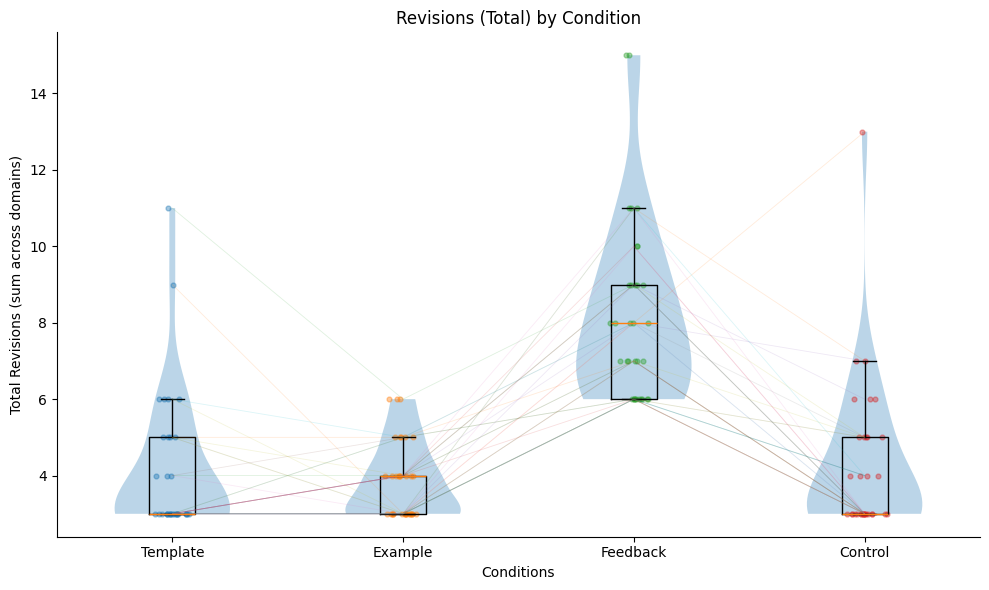
\includegraphics[width=0.7\textwidth]{figures/07.png}
\caption{Distribution of Total Revisions by Assistance Condition}
\label{fig:revision_frequency}
\end{figure}

The violin plot in \autoref{fig:revision_frequency} illustrates the total number of prompt revisions across the four assistance conditions. Revision frequency varied systematically by condition. The Feedback assistance produced the highest number of revisions, with a median of around 8 and several participants exceeding 12 revisions, indicating that iterative refinement was most actively pursued under this condition. The control condition also showed relatively high variability, with some participants making frequent revisions despite the absence of structured support. In contrast, the Template and Example assistance resulted in fewer revisions overall, with medians clustered between three and five edits, reflecting more concise revision behavior. These findings suggest that structured assistance, particularly feedback-based, encouraged participants to engage more extensively in iterative prompt refinement, whereas unguided and template-based conditions led to shorter and less variable revision processes.

\subsubsection{Time on Task Across Assistance Conditions}
\FloatBarrier
\usepackage{:}
\begin{figure}[h]
\centering
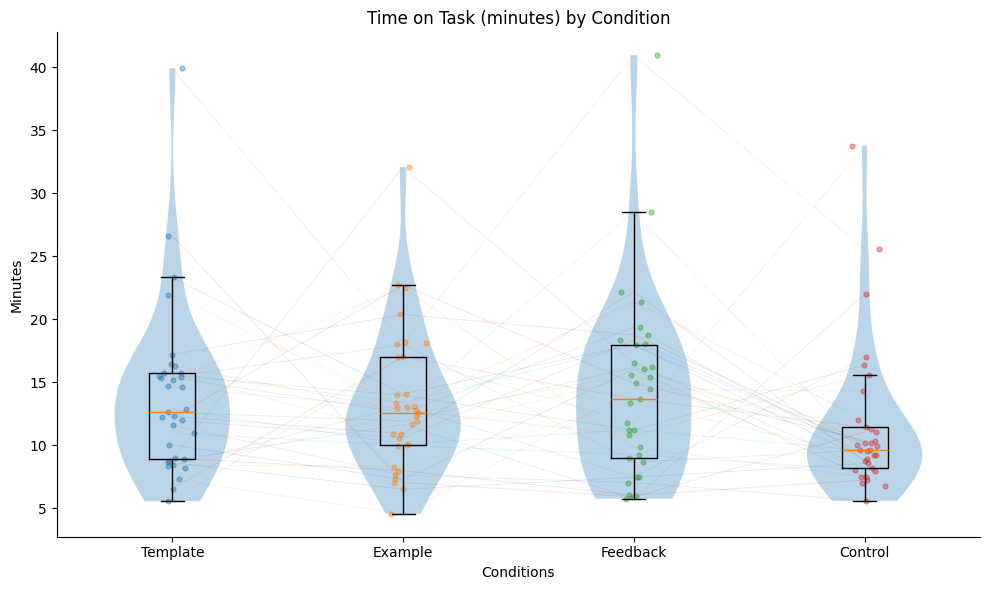
\includegraphics[width=0.7\textwidth]{figures/08.png}
\caption{Distribution of Time on Task (Minutes) by Assistance Condition}
\label{fig:time_on_task}
\end{figure}

In \autoref{fig:time_on_task} time on task varied across assistance conditions, with the Feedback condition showing the highest durations (median $\approx$ 15–18 minutes, with several participants exceeding 30 minutes), suggesting that iterative refinement required additional time. Template-based and example-based assistance showed moderate time investments (medians around 12–14 minutes), while the control condition resulted in the shortest completion times (median $\approx$ 9–10 minutes). These results indicate that structured support, particularly feedback-based guidance, led participants to spend more time engaging with tasks, whereas unguided conditions were completed more quickly but with less iterative depth.

\subsection{\textbf{Correlation Analysis}}

\subsubsection{Spearman's $\rho$ Correlation Analysis:}

We analyzed associations between participant factors (such as, digital literacy, confidence) and outcomes (such as, perceived effectiveness, satisfaction) using Spearman's rank correlation ($\rho$)—a non-parametric measure of monotonic association that does not assume normality and is well suited for ordinal survey data. Unlike Pearson's correlation, which requires interval data and normally distributed residuals, Spearman's $\rho$ operates on ranked data, making it robust against outliers and ties. This test is particularly recommended in survey-based human AI studies where Likert scales dominate and non-normality is common \cite{tyagi2022use,winter2024comparing}.

In the presence of ties, which are inevitable in Likert-scale data, Spearman's $\rho$ is defined as:

\begin{equation}
\rho = \frac{\text{cov}(R_X, R_Y)}{\sigma_{R_X} \, \sigma_{R_Y}}
\end{equation}

where $R_X$ and $R_Y$ are the ranked values of the two variables, $\text{cov}$ denotes covariance, and $\sigma$ indicates the standard deviation of the ranks \cite{upadhyay2021correlation}.

The computation was conducted using \texttt{scipy.stats.spearmanr}, which automatically ranks the data (assigning average ranks for ties), computes the covariance of ranks, and returns both the correlation coefficient and the $p$-value to test the null hypothesis $H_{0}: \rho = 0$. We applied this method to build a full correlation matrix, highlight statistically significant relationships, and visualize them with heatmaps and scatterplots as recommended by recent methodological work \cite{gu2022complex,briganti2024network}.

\begin{figure}[h]
\centering
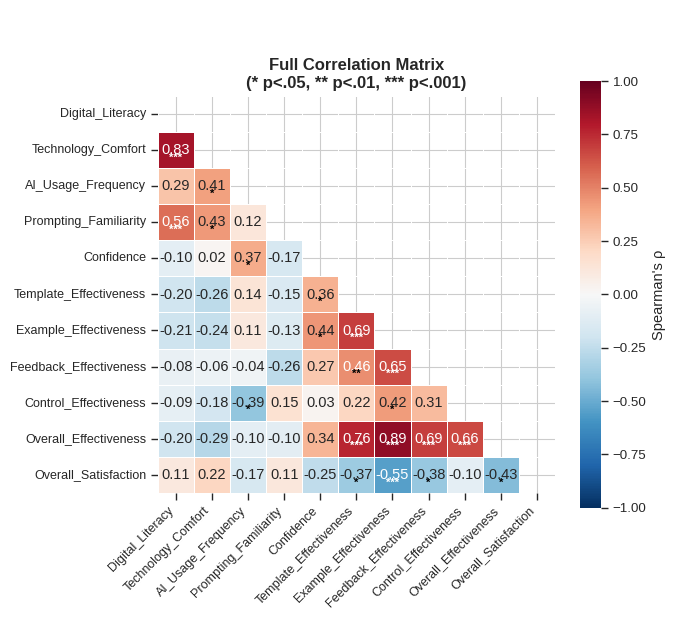
\includegraphics[width=0.65\textwidth]{figures/09.png}
\caption{Spearman Correlation Matrix of Predictor and Outcome Variables}
\label{fig:correlation_matrix}
\end{figure}

\autoref{fig:correlation_matrix} presents the full correlation matrix of participant characteristics and outcome measures. Several meaningful associations were observed. Technology comfort correlated strongly with prompting familiarity ($\rho = 0.83$, ***), indicating that participants more comfortable with technology were also more adept at constructing prompts. Confidence also showed positive associations with effectiveness ratings, particularly for Template ($\rho = 0.36$, *) and Example ($\rho = 0.44$, **), suggesting that self-assured participants benefited more from structured support. Effectiveness scores across conditions were positively interrelated, such as Example and Feedback ($\rho = 0.65$, ***), reflecting consistency in participants' evaluations. Overall effectiveness correlated positively with structured conditions ($\rho = 0.59–0.76$, ***), reinforcing the value of example-based and feedback-based support, while negative associations with individual challenge ratings suggested that stronger assistance reduced perceived difficulty. In contrast, digital literacy displayed only weak, non-significant correlations with outcomes, implying that task-specific confidence and comfort were more predictive of success than general digital skills. Collectively, these findings highlight that structured assistance, especially example-based and feedback-based assistance conditions, was reliably associated with higher effectiveness and satisfaction, moderated by participants' confidence and technology comfort.

\begin{figure}[h]
\centering
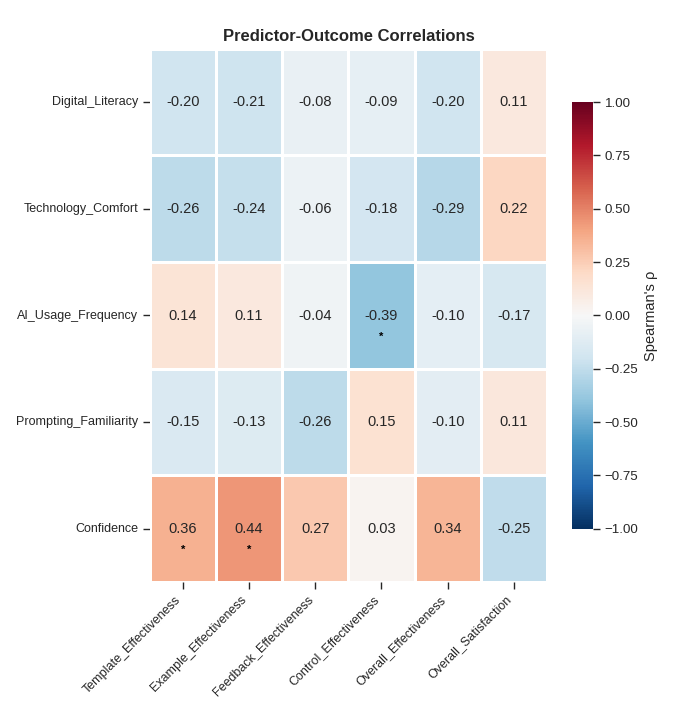
\includegraphics[width=0.4\textwidth]{figures/10.png}
\caption{Predictor Outcome Spearman Correlations}
\label{fig:predictor_outcome}
\end{figure}

\autoref{fig:predictor_outcome} illustrates the correlations between participant characteristics and outcome measures. Confidence emerged as the strongest positive predictor, showing significant associations with Example Effectiveness ($\rho = 0.44$, *), Template Effectiveness ($\rho = 0.36$, *), and Overall Effectiveness ($\rho = 0.34$). This indicates that participants who were more confident tended to produce more effective prompts when supported by structured assistance conditions. In contrast, AI usage frequency correlated negatively with Control Effectiveness ($\rho = –0.39$, *), suggesting that participants with greater prior experience using AI tools rated unguided prompting less favorably. Other predictors, such as technology\_comfort and prompting\_familiarity, displayed only weak, non-significant associations, while digital\_literacy showed negligible relationships with outcomes. Collectively, these findings emphasize that task-specific confidence, rather than general digital skills or technology familiarity, played the most critical role in shaping perceptions of effectiveness and satisfaction with the assistance conditions.


\begin{figure}[h]
\centering
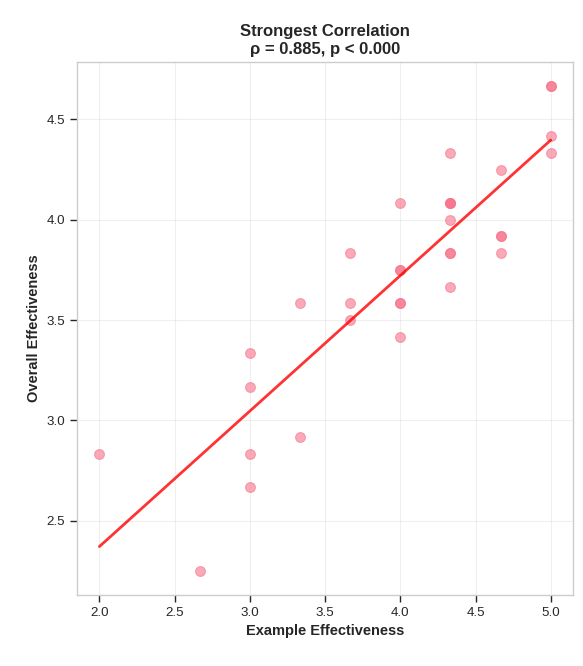
\includegraphics[width=0.3\textwidth]{figures/11.png}
\caption{Strongest Correlation Between Example Effectiveness and Overall Effectiveness}
\label{fig:strongest_correlation}
\end{figure}

\autoref{fig:strongest_correlation} depicts the strongest association observed in the dataset, between Example Effectiveness (x-axis) and Overall Effectiveness (y-axis). The correlation was exceptionally strong ($\rho = 0.885$, $p < .001$), demonstrating a highly significant positive monotonic relationship. The fitted regression line illustrates a clear upward trend, indicating that participants who perceived example-based assistance as more effective also tended to evaluate their overall task performance more positively. This finding underscores that example-based support was not only rated as highly effective within individual tasks but also emerged as the strongest predictor of overall success, highlighting its central role among the assistance conditions.

\begin{figure}[h]
\centering
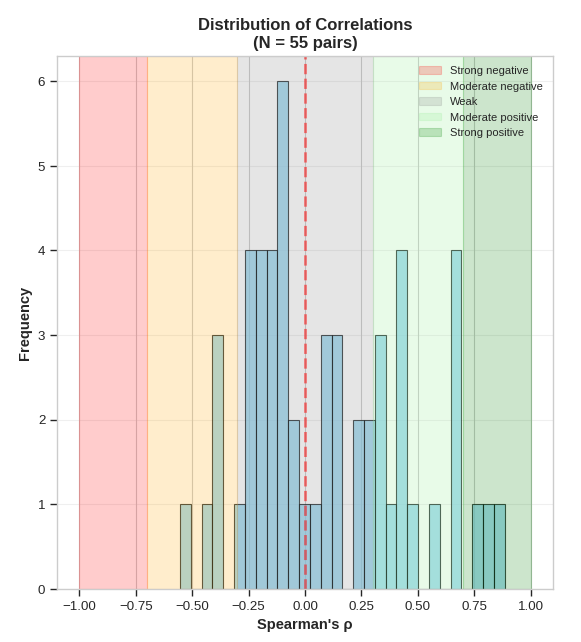
\includegraphics[width=0.4\textwidth]{figures/12.png}
\caption{Distribution of Spearman's Correlation Coefficients Across Variable Pairs}
\label{fig:correlation_distribution}
\end{figure}

\autoref{fig:correlation_distribution} displays the distribution of all 55 Spearman's $\rho$ values calculated across variable pairs in the dataset. The x-axis ranges from –1 (perfect negative association) to +1 (perfect positive association), while the y-axis indicates the frequency of correlations within each bin. Colored bands mark interpretive thresholds, from strong negative ($\rho \leq –0.7$) to strong positive ($\rho \geq 0.7$), with the dashed vertical line denoting zero correlation. Most correlations clustered in the weak to moderate range, suggesting modest associations between participant characteristics and outcomes. A smaller subset of strong positive correlations was observed, particularly those involving example effectiveness, while strong negative associations were rare. This distribution provides an overall perspective on the relational structure of the dataset, complementing the more detailed patterns illustrated by the correlation heatmaps and scatterplots.

% Bibliography references used in the text
\bibliographystyle{plain}
% Note: You would need to add these references to your .bib file
% [22] Benavoli et al. 2016
% [18] In et al. 2024  
% [19] Tomczak & Tomczak 2022
% [29] Tyagi et al. 2022
% [30] Winter et al. 2024
% [31] Upadhyay & Shukla 2021
% [32] Gu 2022
% [33] Briganti et al. 2024